\chapter{Teorija}

Šajā nodaļā tiek apskatīti jaudas pastiprinātāji, to vadības sistēmas, izstarotās un atstarotās jaudas detektori, kā arī piedāvātie risinājumi vadības sistēmām, jaudas detektoriem un izvēlētie risinājumi pastiprinātājam, vadības sistēmai un jaudas noteikšanai.

\section{"Koncepts"}
\subsection{Augstas jaudas RF pastiprinātāji}
Augstas jaudas RF pastiprinātāji ir būtisks sastāvdaļā bezvadu sistēmās. To uzdevums ir pastiprināt signālus jaudu, ļaujot tos pārraidīt lielākos attālumos. Šie pastiprinātāji tiek izmantoti dažādās nozarēs, tostarp satelītu sakaros.

Tipisks augstas jaudas RF pastiprinātājs sastāv no vairākām daļām, kuras veic dažādas signāla pastiprināšanas un kondicionēšanas funkcijas. 

Galvenās sastāvdaļas ir:
\begin{itemize}
    \item Ieejas tīkla saskaņošana;
    \begin{itemize}
        \item Nodrošina maksimālu enerģijas pārnesi no signāla avota uz pastiprinātāju;
        \item Pielāgo ieejas signāla avota pretestību pastiprinātāja pirmajai pakāpei;
    \end{itemize}
    \item Priekšpastiprinātājs;
    \begin{itemize}
        \item Nodrošina sākotnējo signāla pastiprināšanu ar nelielu pastiprinājumu;
        \item Maztrokšnojoša pakāpe;
    \end{itemize}
    \item Vidējās jaudas pastiprinātājs;
    \begin{itemize}
        \item Veic lielāko daļu signāla pastiprināšanas;
        \item Parasti sastāv no vairākām tranzistoru pakāpēm kaskādes vai paralēlā konfigurācijā;
        \item Var ietvert atgriezeniskās saites shēmas linearitātes un stabilitātes uzlabošanai; 
    \end{itemize}
    \item Gala jaudas pastiprinātājs (izejas pakāpe):
    \begin{itemize}
        \item Nodrošina visaugstāko jaudas līmeni, bieži diapazonā no W līdz kW.;
        \item Izmanto augstas jaudas tranzistorus (piem., MOSFET, GaN HEMT vai LDMOS) vai vakuuma lampas;
        \item Jānodrošina efektīvu siltuma izkliedi, jo rada lielu enerģijas zudumu siltumā.
    \end{itemize}
    \item Izejas saskaņošanas tīkls:
    \begin{itemize}
        \item Saskaņo pastiprinātāja izejas pretestību ar slodzi (piem., antenu vai pārraides līniju);
        \item Nodrošina efektīvu jaudas pārnesi un samazina signāla atstarojumus.
    \end{itemize}
    \item Barošanas avoti un darba punkta iestatīšanas shēmas:
    \begin{itemize}
        \item Nodrošina nepieciešamo līdzstrāvas barošanu aktīvajām komponentēm;
        \item Var ietvert sprieguma stabilizatorus, DC-DC pārveidotājus un darba punkta iestatīšanas tranzistoriem.
    \end{itemize}
     \item Dzesēšanas sistēma:
     \begin{itemize}
        \item Izmanto radiatorus, ventilatorus vai šķidruma dzesēšanas sistēmas termiskās stabilitātes nodrošināšanai.
    \end{itemize}
\end{itemize}

Augstas jaudas RF pastiprinātājus var klasificēt pēc to darbības režīma un efektivitātes:
\begin{itemize}
    \item A klase: Augsta linearitāte, bet zema efektivitāte (~25-30\%). Izmanto pielietojumos, kur nepieciešama minimāla signāla kropļošana;
    \item B/AB klase: Uzlabota efektivitāte (~50-70\%) ar nelielu nelinearitāti, bieži lieto apraides raidītājos;
    \item C klase: Augsta efektivitāte (~75-85\%), piemērota pielietojumiem, kur neliela signāla kropļošana nav kritiska, piemēram, FM raidītājos;
    \item D/E/F klase: pastiprinātāji ar efektivitāti virs 90\%, izmanto specializētās RF pielietojumos.
\end{itemize}

% atsauces:
% Pozar, D. M. (2011). Microwave Engineering (4th ed.). Wiley.
% Krauss, H. L., Bostian, C. W., & Raab, F. H. (1980). Solid State Radio Engineering. Wiley.
% Cripps, S. C. (2006). RF Power Amplifiers for Wireless Communications (2nd ed.). Artech House.

\subsection{Vadības sistēmas RF jaudas pastiprinātājiem}
Lai gan RF jaudas pastiprinātāji ir atbildīgi par signāla pastiprināšanu, vadības sistēma ir tā, kas nodrošina to optimālu darbību, precīzu jaudas regulēšanu un aizsardzību pret iespējamiem darbības traucējumiem.
RF jaudas pastiprinātājiem ir nepieciešama vadības sistēma vairāku iemeslu dēļ:
\begin{itemize}
    \item Jaudas regulēšana: RF pastiprinātājiem jāspēj dinamiski pielāgot savu jaudu atkarībā no ārējiem faktoriem, piemēram, signāla kvalitātes, tālāka pārraides attāluma vai apkārtējās vides apstākļiem;
    \item Aizsardzība pret pārslodzi: RF pastiprinātāji var tikt bojāti pārmērīgas jaudas dēļ. Vadības sistēma var uzraudzīt pastiprinātāja darbību un aktivizēt aizsardzības režīmus, piemēram, automātisku izslēgšanu vai jaudas samazināšanu, lai novērstu bojājumus;
    \item Efektivitāte un enerģijas patēriņš: Ar efektīvu vadības sistēmu iespējams uzlabot pastiprinātāja energoefektivitāti, optimizējot darbības apstākļus, samazinot liekās enerģijas patēriņu un palielinot sistēmas darbības ilgumu;
\end{itemize}

RF jaudas pastiprinātāju vadības sistēmas tiek pielietotas vairākās jomās:

\begin{itemize}
    \item Telekomunikācijas - Vadības sistēma palīdz pielāgot jaudu atbilstoši tīkla apstākļiem, lai nodrošinātu optimālu pārraidi un izvairītos no traucējumiem;
    \item Kosmosa un satelītu tehnoloģijas - Vadības sistēma ļauj uzraudzīt jaudas līmeni un pielāgot to, ņemot vērā vides apstākļus, piemēram, atmosfēras traucējumus;
    \item Radar sistēmas - Vadības sistēma nodrošina, ka radarā tiek izmantota optimāla jauda, lai uzlabotu precizitāti un samazinātu traucējumus;
    \item RFID un bezvadu sensoru tīkli - Vadības sistēma palīdz regulēt jaudu un nodrošina efektīvu enerģijas patēriņu.;
\end{itemize}

Vadības sistēmas RF jaudas pastiprinātājiem tiek implementētas vairākos veidos:
\begin{itemize}
    \item Automātiskā jaudas regulēšana (AGC) - AGC ir bieži izmantota tehnoloģija, kas ļauj automātiski pielāgot pastiprinātāja jaudu, lai uzturētu optimālu signāla līmeni;
    \item Digitālie signālu procesori (DSP) - Vadības sistēmas bieži izmanto DSP tehnoloģijas, lai apstrādātu un analizētu RF signālus reālajā laikā. DSP ļauj veikt precīzu signāla analīzi un uzraudzību, kas nepieciešama, lai regulētu jaudu un nodrošinātu augstu pārraides kvalitāti;
    \item Vairāku sensoru izmantošana - Lai uzraudzītu dažādus parametrus, piemēram, temperatūru, spriegumu un strāvu, tiek izmantoti vairāki sensori, kas darbojas kopā ar vadības sistēmu, lai nodrošinātu pastiprinātāja aizsardzību un efektīvu darbību;
    \item Kompleksi algoritmi un kontrolējošas loģikas sistēmas - Vadības sistēmas var ietvert algoritmus, kas ņem vērā daudzus faktorus, piemēram, apkārtējo traucējumu līmeni, sistēmas pieprasījumu un jaudas pieejamību. Šie algoritmi ļauj pielāgot pastiprinātāja darbību un uzlabot sistēmas veiktspēju;
\end{itemize}

RF jaudas pastiprinātāji ir svarīgi sastāvdaļa modernās komunikāciju sistēmās, un to efektīva darbība ir atkarīga no labi izstrādātām vadības sistēmām. Šādas sistēmas nodrošina jaudas regulēšanu, aizsardzību, enerģijas efektivitāti un augstu signāla kvalitāti, kas ir nepieciešama daudzās nozarēs, sākot no telekomunikācijām līdz kosmosa tehnoloģijām. Ar vienkāršotu.

\subsection{Teorētiska un tehniskā skaidrojums par izstaroto un atstarotā jaudas detektoriem (Prefl un Pfwd detektoriem)}
P\textsubscript{refl} un P\textsubscript{fwd} noteikšanas shēmas tiek izmantotas RF sistēmās, lai uzraudzītu izstaroto un atstaroto jaudu pārvades līnijā. Šie mērījumi ir būtiski, lai nodrošinātu, ka sistēma darbojas efektīvi. P\textsubscript{refl} attiecas uz atstaroto jaudu uz jaudas pastiprinātāju un P\textsubscript{fwd} attiecas uz izstaroto jaudu no jaudas pastiprinātāja.

\subsubsection{Atstarotās P\textsubscript{refl} jaudas detektori}
Atstarotā jauda ir signāla daļa, kas tiek atgriezta avotā pretestības neatbilstību vai atstarojumu dēļ pārraides līnijā. Atstarotās jaudas noteikšana ir svarīga, lai nodrošinātu, ka sistēma nepiedzīvo ievērojamus zaudējumus atstarošanas dēļ, kas var sabojāt komponentes vai izraisīt neefektivitāti.

Atstarotās jaudas detektora tipi:
\begin{itemize}
    \item \textbf{Uz virziena savienotāju balstīta noteikšana (Directional Coupler-based Detection)};
\end{itemize}

Virziena savienotājs ir visizplatītākā metode atstarotās jaudas mērīšanai. Tas ņem paraugus no nelielas atstarotā signāla daļas un novirza to uz detektoru, parasti diodi vai RF barošanas sensoru.

Virziena savienotājs sadala tajā ienākošo jaudu divos ceļos. Signāls, kas pārvietojas virzienā uz priekšu, tiek savienots no viena porta (izstarotā jauda), bet atstarotais signāls tiek savienots no cita porta (atstarotā jauda). Šo jaudu attiecību nosaka savienotāja konstrukcija, un atstarotā jauda tiek noteikta caur saistītu portu, kas atbilst atstarojumam.
Priekšrocības:
\begin{itemize}
    \item Precīzs un vienkāršs;
    \item Nodrošina vienlaicīgus izstarotā un atstarotā jaudas mērījumus;
    \item Bieži un plaši izmanto sakaru sistēmās.
\end{itemize}
Mīnusi:
\begin{itemize}
    \item Frekvences reakcija ir atkarīga no savienotāja konstrukcijas;
    \item Savienotāja zudums (insertion loss) var samazināt mērījumu precizitāti.
\end{itemize}

\begin{itemize}
    \item \textbf{(Bridge-based Detection [Wheatstone Bridge or Impedance Bridge])};
\end{itemize}
Šī metode izmanto tilta slēgumu, lai izmērītu atstaroto jaudu. Šādās ķēdēs atstarošana izraisa sprieguma nelīdzsvarotību, ko var noteikt, bieži vien izmantojot diodi vai citu taisngriešanas elementu.

Līdzsvarota tilta slēgumā izmanto pretestības saskaņošanas principu, lai noteiktu atstarojumus. Ja nav atspulga (perfekta atbilstība), tilts ir līdzsvarots, un signāla atšķirība neveidojas. Kad rodas atstarojumi, pretestības neatbilstība izraisa nelīdzsvarotību.

Priekšrocības:
\begin{itemize}
    \item Augsta jutība pret nelielām atstarotās jaudas variācijām;
    \item Var strādāt plašā frekvenču diapazonā.
\end{itemize}
Mīnusi:
\begin{itemize}
    \item Augstāka sarežgītība salīdzinot ar citām metodēm;
    \item Jutīgi pret dreifēšanu, īpaši ar temperatūras izmaiņām.
\end{itemize}

\begin{itemize}
    \item \textbf{Diožu jaudas detektori (Diode-based Detectors)}.
\end{itemize}
Vienkāršu diodes detektoru var izmantot kopā ar virziena savienotāju vai tiltu, lai tieši izmērītu atstaroto jaudu.

Diodes taisngriezis uztver RF signālu un pārvērš to līdzstrāvas signālā, ko var izmērīt ar atbilstošu skaitītāju. Līdstrāvas spriegums ir proporcionāls atstarotā signāla jaudas līmenim.

Priekšrocības:
\begin{itemize}
    \item Vienkāršā un rentabla (cost-effective);
    \item Nodrošina atstarotās jaudas mērīšanu reālā laikā.
\end{itemize}
Mīnusi:
\begin{itemize}
    \item Precizitāti ierobežo diodes nelinearitāte, īpaši lieljaudas signāliem;
\end{itemize}

\subsubsection{Izstarotās P\textsubscript{fwd} jaudas detektori}
Izstarotā jauda tiek piegādāta no avota uz antenu vai citu patērētāju. Ir nepieciešams monitorēt izstaroto jaudu, lai novērtētu jaudas pastiprinātāja pastiprinājuma koeficientu un vai darbība ir optimāla.

\begin{itemize}
    \item \textbf{Termiskās jaudas noteicējs (Thermal Power Detectors)};
\end{itemize}
Šie detektori mēra signāla radīto siltumu, kad tas iet caur pretestību. Sildīšanas efekts ir proporcionāls piegādātajai jaudai, un termistors vai termopāris var pārvērst šo temperatūras maiņu lasāmā signālā.

Termiskais detektors mēra temperatūras paaugstināšanos pretestībā, ko izraisa RF signāla izkliedētā jauda. Šī metode ir diezgan precīza, jo tā tieši mēra faktisko jaudu, taču tā relatīvi lēna, un tai nepieciešama rūpīga kalibrēšana.

Priekšrocības:
\begin{itemize}
    \item Precīzs un nodrošina absolūtus jaudas mērījumus;
    \item Var izmērīt gan  izstaroto, gan atstaroto jaudu.
\end{itemize}
Mīnusi:
\begin{itemize}
    \item Lēns reakcijas laiks, kas neatļauj izmantot augstās frekvenču aplikācijās.;
\end{itemize}

\begin{itemize}
    \item \textbf{Diožu jaudas detektori (Diode-based Detectors)};
\end{itemize}
Līdzīgi kā atstarotās jaudas noteikšanā, arī izstaroto jaudu var noteikt, taisngriežot signālu, izmantojot diodes. Signāla ceļā tiek ievietots diodes detektors, un, tā kā diode taisno RF signālu, iegūtais līdzstrāvas spriegums ir proporcionāls momentānajai jaudai.

Priekšrocības:
\begin{itemize}
    \item Vienkārši un lēti;
    \item Ātrs reakcijas laiks.
\end{itemize}
Mīnusi:
\begin{itemize}
    \item Precizitāti var ierobežot diodes īpašības, īpaši augstfrekvences signāliem;
    \item Nepieciešama kalibrēšana dažādiem signālu tipiem.
\end{itemize}

\begin{itemize}
    \item \textbf{Pīķa detektori (Peak Detectors)}.
\end{itemize}
Pīķa detektorus var izmantot sistēmās, kurās jāuzrauga tikai maksimālā jauda. Šie detektori uztver maksimālo momentāno jaudu, bieži izmantojot diodes un kondensatora kombināciju, lai saglabātu maksimālo vērtību.

Maksimālais detektors uztver un notur ieejas signāla maksimālo vērtību. Kad signāls sasniedz maksimumu, kondensators uzlādējas līdz noteiktam spriegumam, un līdzstrāvas izeja atspoguļo maksimālo jaudas līmeni.

Priekšrocības:
\begin{itemize}
    \item Ātra reakcija un precīzi pīķa mērījumi;
    \item Noderīga signāliem ar pārejošiem impulsu RF signāliem.
\end{itemize}
Mīnusi:
\begin{itemize}
    \item Nenodrošina vidējo jaudas vērtību;
    \item Var būt mazāk efektīvs nepārtrauktiem signāliem bez būtiskiem pīķiem.
\end{itemize}

Kuras metodes izmanto kādiem pielietojumiem:
\begin{itemize}
    \item Komunikācijas sistēmās - Uz virziena savienotāju balstīta noteikšana (Directional Couplers);
    \item Augstas jaudas sistēmās (raidītājos, jaudas pastiprinātājos) - Termiskais detektors(Thermal Detectors);
    \item Signāla monitorēšanai un atkļūdošanai - Diožu detektors (Diode-base detector);
    \item Mērījumu iekārtām - Tilta detektori (Bridge-based detection circuits).
\end{itemize}

%atsauces
% Gupta, R. S., & Wadhwa, M. (2014). "Microwave Engineering." - This text provides detailed theoretical explanations and practical applications for various types of RF power detectors, including directional couplers and diode detectors.
% Pozar, D. M. (2012). "Microwave Engineering" (4th ed.). - Offers an in-depth explanation of impedance matching and directional coupler theory, relevant to reflected and forward power detection.
% Krauss, J. D. (2011). "RF and Microwave Radiation Safety." - Covers methods and challenges in power measurement, including forward and reflected power detection in RF systems.

\section{"Apskatītie risinājumi"}
\subsection{Vadības integrālās shēmas priekš jaudas pastiprinātāji}
\begin{table}[h]
    \centering
    \renewcommand{\arraystretch}{1.3}
    \setlength{\tabcolsep}{5pt} % Adjust column spacing
    \begin{adjustbox}{max width=\textwidth}
    \begin{tabular}{|p{3cm}|p{3cm}|p{3cm}|p{3cm}|p{4cm}|}
        \hline
        \textbf{Integrālā shēma} & \textbf{Funkcijas} & \textbf{Pielietojums} & \textbf{Spriegums} & \textbf{Atšķiras} \\
        \hline
        Analog Devices AD7293 & Darba punkta iestatīšana un aizsardzība & RF pastiprinātāju vadība, signālu uzraudzība un aizsardzība & 3.3V -- 5.5V & Integrēts ADC un DAC, termālā aizsardzība, sprieguma un strāvas uzraudzība, trauksmes izvadi \\
        \hline
        Texas Instruments ADC12D1800 & 12-Bitu, 1.8 GSPS Datu pārveidotājs & RF sistēmas ātrai signālu nolasei un uzraudzībai & 3.3V & Ātra nolase, zems enerģijas patēriņš un augsta nolases izšķirtspēja \\
        \hline
        Maxim MAX11200 & 24-Bitu, 4-kanālu ADC ar iebūvētu multiplikatoru & Signālu iegūšanai RF pastiprinātāju vadībā & 2.7V -- 5.5V & Augsta precizitāte, zema enerģija, integrēta multiplikatora funkcionalitāte \\
        \hline
        Analog Devices AD5700 & 16-Bitu, 4-kanālu signālu iegūšanas sistēma & RF sistēmu signālu mērīšanai un kontrolei & 3.0V -- 5.5V & Precīzi signālu mērījumi, integrēti trauksmes izvadi, termālā aizsardzība \\
        \hline
        Linear Technology LTC2378-16 & 16-Bitu, 8-kanālu ADC ar iebūvētu multiplikatoru & RF signālu mērīšanai un uzraudzībai & 2.7V -- 5.5V & Augsta precizitāte, zema trokšņa veiktspēja, integrēti trauksmes izvadi \\
        \hline
        Maxim MAX14733 & 16-Bitu, vairāku kanālu ADC ar iebūvētu multiplikatoru & RF signālu uzraudzībai un vadības sistēmām & 3.0V -- 5.5V & Vairāku kanālu signālu iegūšana, zems trokšņu līmenis, trauksmes izvadi \\
        \hline
        Texas Instruments ADS8900B & 16-Bitu, vienkanālu, zema enerģijas ADC & Precīzai signālu uzraudzībai RF pastiprinātāju vadībā & 2.7V -- 5.5V & Zems aizkaves laiks, programmējami trauksmes sliekšņi un reālā laika monitorēšanai \\
        \hline
        Analog Devices AD7779 & 24-Bitu, vairāku kanālu Sigma-Delta ADC ar trauksmes izvadiem & RF sistēmu signālu uzraudzībai un vadībai & 2.7V -- 5.5V & Augsta izšķirtspēja un precizitāte, vairāku kanālu atbalsts, integrēti trauksmes izvadi \\
        \hline
    \end{tabular}
    \end{adjustbox}
    \caption{GaN pastiprinātāju vadības bloku mikroshēmu piemēri un salīdzinājums}
    \label{tab:gan_control_blocks}
\end{table}

No apskatītajiem RF jaudas vadības integrālajām shēmām tika  izvēlēta Analog Devices ražojums "AD7293" salīdzinoši lētās izmaksas dēļ un nodrošina visu nepieciešamo funkcionalitāti pēc VSRC specifikācijām.

\subsection{Izstarotās un atstarotājs jaudas aktīvās RMS jaudas detektors (true RMS power detector)}
Virziena savienotāji izmanto, lai izmērītu gan izstaroto, gan atstaroto jaudu. Virziena savienotājs ir pasīva četru portu ierīce, kas ļauj enerģiju no vienas pārvades līnijas kontrolētā veidā pārnest uz otru pārvades līniju. Tas atdala signālu divās komponentēs: viens ir izstarotā jauda (plūst tajā pašā virzienā kā signāls), bet otrs ir atstarotā jauda (kas plūst atpakaļ uz avotu, ja ir pretestības neatbilstība).

Virziena savienotājs sastāv no četriem portiem:
\begin{itemize}
    \item Ieejas ports - Tas ir ports, kurā signāls tiek ievadīts savienotājā no raidītāja;
    \item Izejas ports - Ieejas signāla izeja, kas tiek nogādāta uz patērētāju, piemēram, antēnu.
    \item Saistīts port (coupled port) - Šī ir pieslēgvieta, kas ir proporcionāls ieejas jaudai. Tas mēra tiešo jaudu līnijā.
    \item Atsaistīts ports (isolated port) - Šis ports saņem atstaroto signālu, kas ir proporcionāla atstarotajam signālam.
\end{itemize}

Darbības princips:
\begin{itemize}
    \item Izejošās jaudas noteikšānai - Ievades signāls nonāk 1. portā, un lielākā daļa no tā iziet no 2. porta. Neliela signāla daļa tiek padota uz 3 portu.
    \item Atstarotās jaudas noteikšānai - Atstarotā jauda ceļo atpakaļ savienotāju, kur daļa no tā tiek padota 4 portā.
\end{itemize}

Virziena savienotāji balstās uz jaudas dalīšanas un savienošanas principu, izmantojot elektromagnētiskos laukus. Šie savienotāji ir paredzēti darbam plašā frekvenču diapazonā, un saites koeficients (coupling factor) nosaka jaudas daudzumu, kas tiek pārnests uz savienoto portu.

\begin{itemize}
    \item \textbf{saites koeficients}
\end{itemize}
Saites koeficients nosaka, cik liela daļa signāla ir "savienota" no galvenās pārraides līnijas uz savienoto līniju. To parasti izsaka dB (decibelos). Piemēram, 20 dB savienotājs nodod 1/100 daļu no ieejas jaudas uz savienoto portu.
Saites koeficientu definē šādi:
\[
C = 10log(\frac{Pinput}{Pcoupled})
\]
, kur
\begin{itemize}
    \item Pinput ir savienotāja ieejas jauda.
    \item Pcoupled ir jauda, kas savienota ar portu 3 (tiešajai jaudai) vai portu 4 (atstarotai jaudai)
\end{itemize}

\begin{itemize}
    \item \textbf{Virziens}
\end{itemize}
Virzība ir vēl viens kritisks parametrs virziena savienotājiem. Tas norāda, cik efektīvi savienotājs atdala izstaroto un atstarotos signālus. Jo augstāks ir virziens.

Virzību parasti izsaka dB un definē kā saistītās jaudas attiecību starp 3 un 4 portu. Ideālā gadījumā savienotājam ar augstu virzību būs niecīgi traucējumi no atstarotā signāla, mērot uz izstaroto jaudu.

\[
D = 10log(\frac{Pcoupledfromport4}{Pcoupledfromport3})
\]

\begin{itemize}
    \item \textbf{Pretestības saskaņošana}
\end{itemize}
Pretestības saskaņošana starp portiem ir būtiska efektīvai signāla pārvadei. Ideālos apstākļos savienotājs ir konstruēts tā, lai ieejas un izejas porti (1. un 2. ports) būtu saskaņoti ar avota un slodzes pretestību (parasti 50 Ω), samazinot atstarojumus savienotājā. Jebkura pretestības neatbilstība palielina atstaroto jaudu, kas var pasliktināt jaudas mērījumu precizitāti.
\begin{itemize}
    \item \textbf{Pārvades līnija}
\end{itemize}
Virziena savienotājs darbojas, izmantojot pārvades līnijas savienojumu, kur divas pārvades līnijas ir novietotas cieši kopā tā, lai elektromagnētiskie lauki no vienas līnijas ietekmētu otru līniju. Sasaistes mehānisma pamatā ir pārvades līniju savstarpējā induktivitāte. Signāli no 1. porta inducē strāvas savienotajā līnijā (3. vai 4. ports), kas ir proporcionāli ieejas jaudai.

\begin{itemize}
    \item \textbf{Jaudas mērīšana}
\end{itemize}

RMS jaudas detektori parasti izmanto virziena savienotājos, lai izmērītu gan uz izstaroto, gan atstaroto jaudu pārvades līnijā. RMS detektors precīzi mēra jaudu, pārveidojot RF signālu līdzstrāvas spriegumā, un pēc tam mērījums tiek apstrādāts, lai noteiktu patieso vidējo jaudu laika gaitā, ņemot vērā gan signāla lielumu, gan fāzi.

Praktiskās sistēmās RMS jaudas detektoru var izmantot, lai izmērītu nesinusoidālus signālus vai signālus ar dažādām amplitūdām.

Virziena savienotāji tiek plaši izmantoti jaudas uzraudzībai un kontrolei RF sistēmās. Daži no pielietojumiem:
\begin{itemize}
    \item Atstarotās jaudas mērīšana.
    \item Izstarotās jaudas mērītāji.
    \item VSWR (sprieguma stāvošo viļņu attiecība) mērījums - Izstaroto un atstarotās jaudas attiecību, kas pazīstama kā VSWR, var aprēķināt, izmantojot mērījumus no virziena savienotāja. Augsts VSWR norāda uz sliktu pretestības atbilstību, kas var izraisīt jaudas zudumus un neefektivitāti;
\end{itemize}

Priekšrocības:
\begin{itemize}
    \item Vienlaicīga izstarotā un atstarotās jaudas mērīšana;
    \item Plašs frekvenču diapazons - Daudzi virziena savienotāji ir paredzēti darbam plašā frekvenču diapazonā;
    \item Uzticamība un precizitāte - nesatur aktīvas komponentes (sastāv no pasīvajām);
    \item Rentablu (cost-effective) - Lēti salīdzinot ar citām metodēm, kur tiek izmantots aktīvi elementi.
\end{itemize}
Mīnusi:
\begin{itemize}
    \item Ievietošanas zudums (insertion loss) - Savienotāja klātbūtne pārvades līnijā rada nelielu zudumu, samazinot kopējo sistēmas efektivitāti.
    \item Pretestības neatbilstība - Ja virziena savienotājs nav pareizi pieskaņots sistēmai, atstarojumi var rasties pašā savienotājā, ietekmējot mērījumu precizitāti;
\end{itemize}

Virziena savienotāji darbojas, pamatojoties uz elektromagnētiskās principiem, un ir ļoti svarīgi tādiem lietojumiem kā jaudas uzraudzība, pretestības saskaņošana un sistēmas diagnostika. Apvienojumā ar True RMS detektoriem tie nodrošina ļoti precīzus jaudas mērījumus signāliem ar dažādām amplitūdām, padarot tos būtiskus sistēmas efektivitātes uzturēšanai un pretestības neatbilstības izraisītu bojājumu novēršanai. Virziena savienotāju priekšrocības, tostarp vienlaicīga mērīšana, augsta virzība un plašs frekvenču diapazons, padara tos par izvēles iespēju daudzās RF pielietojumos, neskatoties uz to ierobežojumiem ievietošanas zudumā un dinamiskajā diapazonā.

\section{"Izvēlētais risinājums"}
\subsection{X-joslas jaudas pastiprinātājs}
\begin{figure}[H]
	\centering
    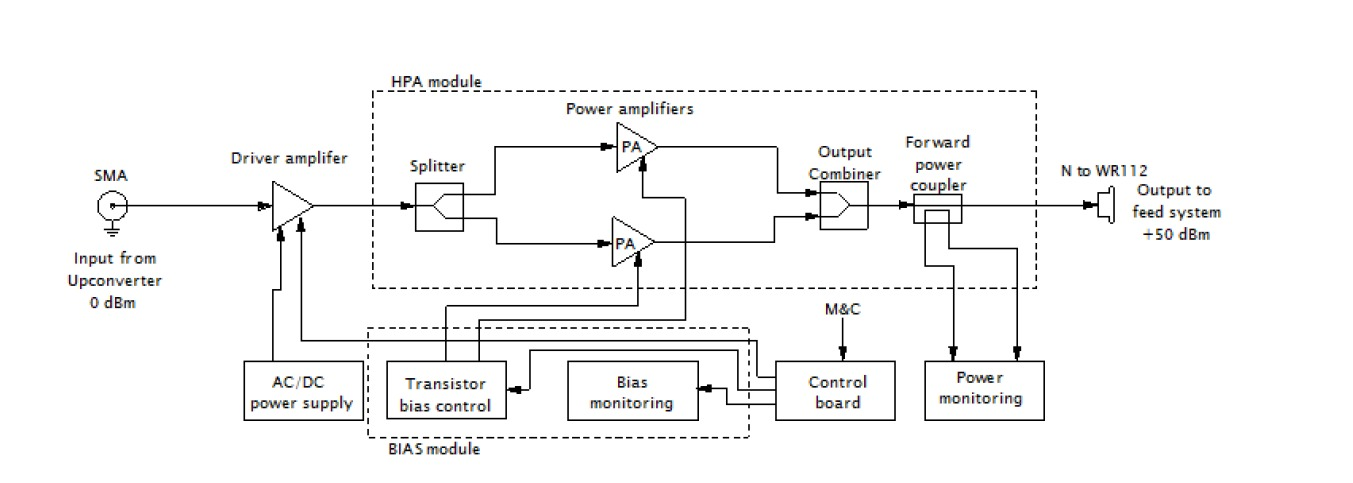
\includegraphics[width=0.9\textwidth]{bildes/HPA.jpg}\hspace{1cm}
    \caption{HPA augsta līmeņa blokshēma}
\end{figure}
(Informācija no M. Bleidera).
\subsection{Monitoringa sistēmas jaudas pastiprinātājiem}

\subsection{Aktīvā vidējā kvadrātiskā vērtības jaudas noteikana}